\documentclass[conference]{IEEEtran}
\IEEEoverridecommandlockouts

\usepackage{graphicx}
\usepackage{booktabs}
\usepackage{array}
\usepackage{url}
\usepackage[hidelinks]{hyperref}

\title{Verifier-Bounded Repair for Safer Retrieval-Augmented Generation}

\author{
\IEEEauthorblockN{Mehmet Can Özen}
\IEEEauthorblockA{Student ID: 20210808020\\
Large Language Models Course Project\\
GitHub: \url{https://github.com/mehmetcanozen/llmtermproject}}
}

\begin{document}
\maketitle

\begin{abstract}
Retrieval-augmented generation (RAG) systems can produce answers with citations that appear authoritative even when the cited passage does not support the claim. This project builds a local citation-grounded RAG pipeline and evaluates whether deterministic verification plus one-step evidence-only repair can improve useful answer coverage without accepting unsupported citations. The system compares a deterministic baseline, an attention-gated variant, a verifier projection, and a new \textit{repair-plus-verifier} variant. On a fixed evaluation split of 200 ASQA examples and 100 synthetic finance questions, the best 3B repair-plus-verifier system keeps unsupported non-abstained answers at 0.0\%, improves finance exact-answer accuracy from 62.0\% to 80.0\%, and improves ASQA short-answer coverage from 26.1\% under verifier projection to 33.5\%. A generated distractor stress test also keeps unsupported accepted answers at 0.0\%. The result is a practical local RAG safety pattern: repair may recover supported answers, but verification remains the final acceptance boundary.
\end{abstract}

\section{Problem and Motivation}
RAG is commonly used to make LLM answers auditable by attaching source citations. A dangerous failure mode is citation hallucination: the model gives a fluent answer and appends a citation marker even though the cited passage does not support the claim. This failure is especially important in legal, medical, or financial settings because the citation surface can make a wrong answer look trustworthy.

The original project proposal targeted deterministic citation enforcement through inference-time grounding signals. The final implementation keeps that goal but shifts toward a fully reproducible local pipeline: deterministic generation, hybrid retrieval, attention-gate instrumentation, a deterministic verifier, and an evidence-only repair loop. The key research question is: can verifier-bounded repair recover answer coverage while maintaining zero unsupported accepted cited answers?

\section{Data and Task}
The project uses two complementary evaluation sources. First, ASQA is used as a bounded local-corpus citation task. The fixed ASQA evaluation split contains 200 examples selected from the local prepared ASQA dev set. Second, a synthetic finance dataset contains 100 fixed questions over fictional disclosures. Finance is useful because exact company, fiscal period, metric type, numeric value, and cited passage ID can be checked deterministically.

The project also includes a generated distractor stress test. In this setting, each prompt receives one additional plausible but irrelevant fourth passage. This stress test is reported separately from the formal fixed split.

\section{LLM Methodology}
The implementation is a Windows-first local RAG pipeline. Retrieval combines dense BGE embeddings with BM25 ranking. The generation models are Qwen2.5-Instruct 3B and 7B run deterministically. The prompt requires every factual sentence to end with citation markers such as \texttt{[P1]}.

Four systems are compared:
\begin{itemize}
\item \textbf{Baseline}: deterministic RAG generation with required citations.
\item \textbf{Gate-only}: baseline plus passage-directed attention tracing and an abstention gate.
\item \textbf{Gate-plus-verifier}: gate outputs projected through deterministic verifier rejection.
\item \textbf{Repair-plus-verifier}: generate, verify, attempt one evidence-only repair if needed, verify again, and otherwise abstain.
\end{itemize}

The verifier is the final acceptance boundary. For finance, it checks company, period, metric, numeric value, and expected cited passage. For ASQA, it checks citation structure, cited-passage existence, explicit anchors, and short-answer coverage. If verification fails after repair, the system outputs \texttt{INSUFFICIENT\_SUPPORT}.

\section{Experiments and Results}
Table~\ref{tab:fixed} summarizes the fixed-split results. The best system is repair-plus-verifier 3B: it preserves 0.0\% unsupported non-abstained answers while improving finance coverage and exact accuracy. Compared with gate-plus-verifier, finance exact accuracy improves from 62.0\% to 80.0\%, and abstention decreases from 53.0\% to 35.0\%. On ASQA, answer coverage is close to verifier projection, while short-answer coverage improves from 26.1\% to 33.5\%.

\begin{table}[t]
\centering
\caption{Fixed-split results. UNS = unsupported non-abstained.}
\label{tab:fixed}
\small
\begin{tabular}{llrrrr}
\toprule
System & Data & N & Cov. & UNS & Abst.\\
\midrule
Baseline 3B & ASQA & 200 & 49.5 & 3.5 & 47.0\\
Gate 3B & ASQA & 200 & 54.5 & 2.5 & 43.0\\
Gate+Ver. 3B & ASQA & 200 & 54.5 & 0.0 & 45.5\\
Repair+Ver. 3B & ASQA & 200 & 53.0 & 0.0 & 47.0\\
Repair+Ver. 7B & ASQA & 200 & 42.5 & 0.0 & 57.5\\
\midrule
Baseline 3B & Fin. & 100 & 47.0 & 1.0 & 52.0\\
Gate+Ver. 3B & Fin. & 100 & 47.0 & 0.0 & 53.0\\
Repair+Ver. 3B & Fin. & 100 & 65.0 & 0.0 & 35.0\\
Repair+Ver. 7B & Fin. & 100 & 0.0 & 0.0 & 100.0\\
\bottomrule
\end{tabular}
\end{table}

\begin{figure*}[t]
\centering
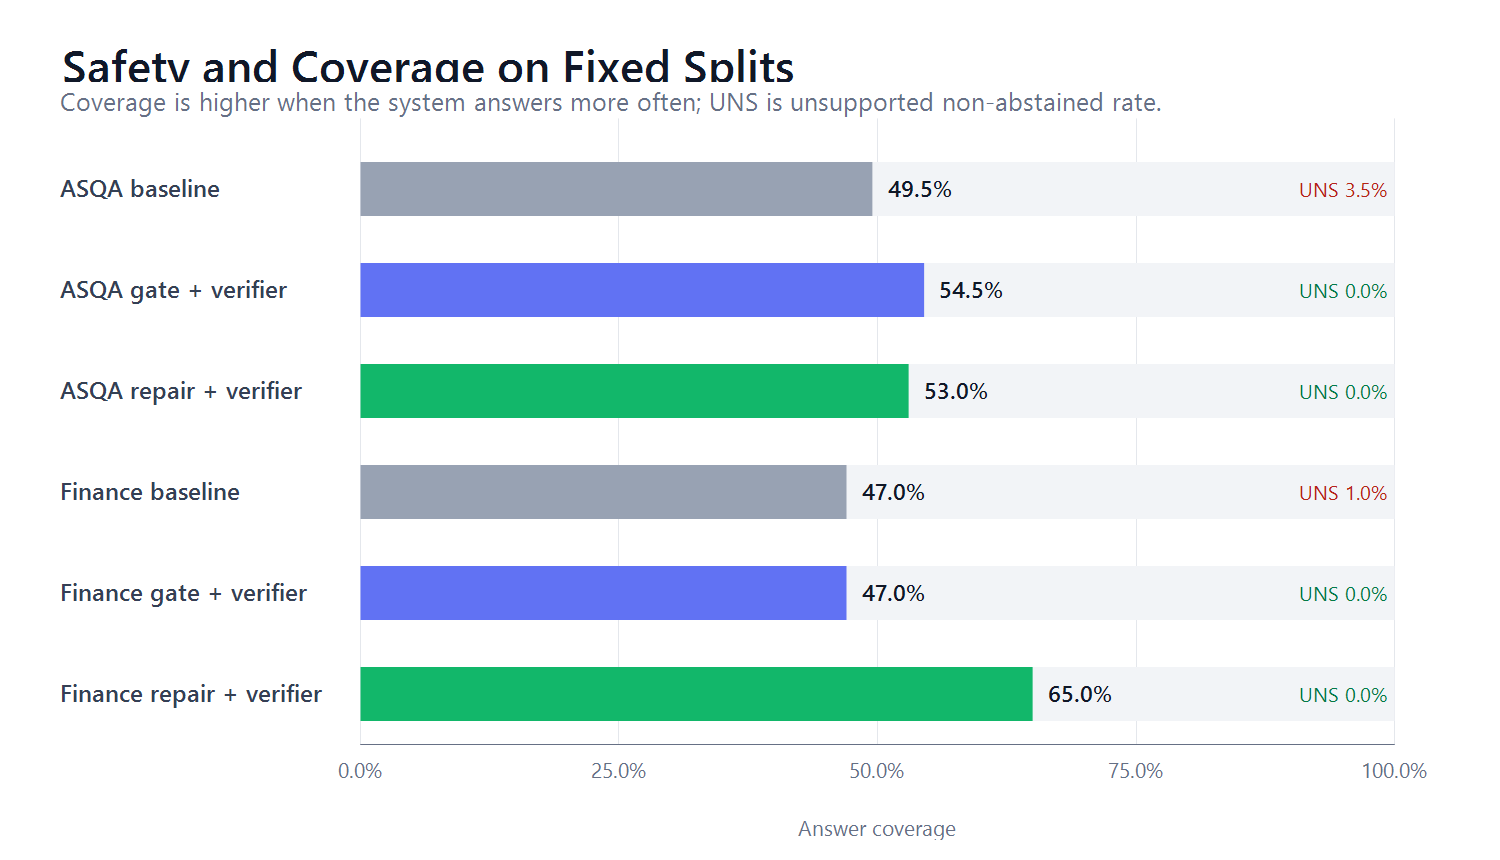
\includegraphics[width=0.98\textwidth]{assets/safety_vs_coverage_frontier.png}
\caption{Fixed-split safety and coverage. Green repair-plus-verifier rows keep unsupported non-abstained output at 0.0\% while improving the strongest utility metrics, especially finance answer coverage.}
\label{fig:frontier}
\end{figure*}

The repair funnel in Table~\ref{tab:repair} shows why the result is more interesting than simple verifier abstention. On finance 3B, 42 examples required repair and 41 were accepted after repair, with 0 unsupported accepted repairs. On ASQA 3B, 24 examples required repair and 11 were accepted. The repair mechanism therefore recovers supported answers while keeping the verifier boundary intact.

\begin{table}[t]
\centering
\caption{Repair salvage results. UAR = unsupported accepted repairs.}
\label{tab:repair}
\small
\begin{tabular}{llrrrr}
\toprule
Data & Model & Attempts & Saved & Salvage & UAR\\
\midrule
ASQA & 3B & 24 & 11 & 45.8 & 0\\
ASQA & 7B & 49 & 11 & 22.4 & 0\\
Finance & 3B & 42 & 41 & 97.6 & 0\\
Finance & 7B & 59 & 44 & 74.6 & 0\\
\bottomrule
\end{tabular}
\end{table}

\begin{figure*}[t]
\centering
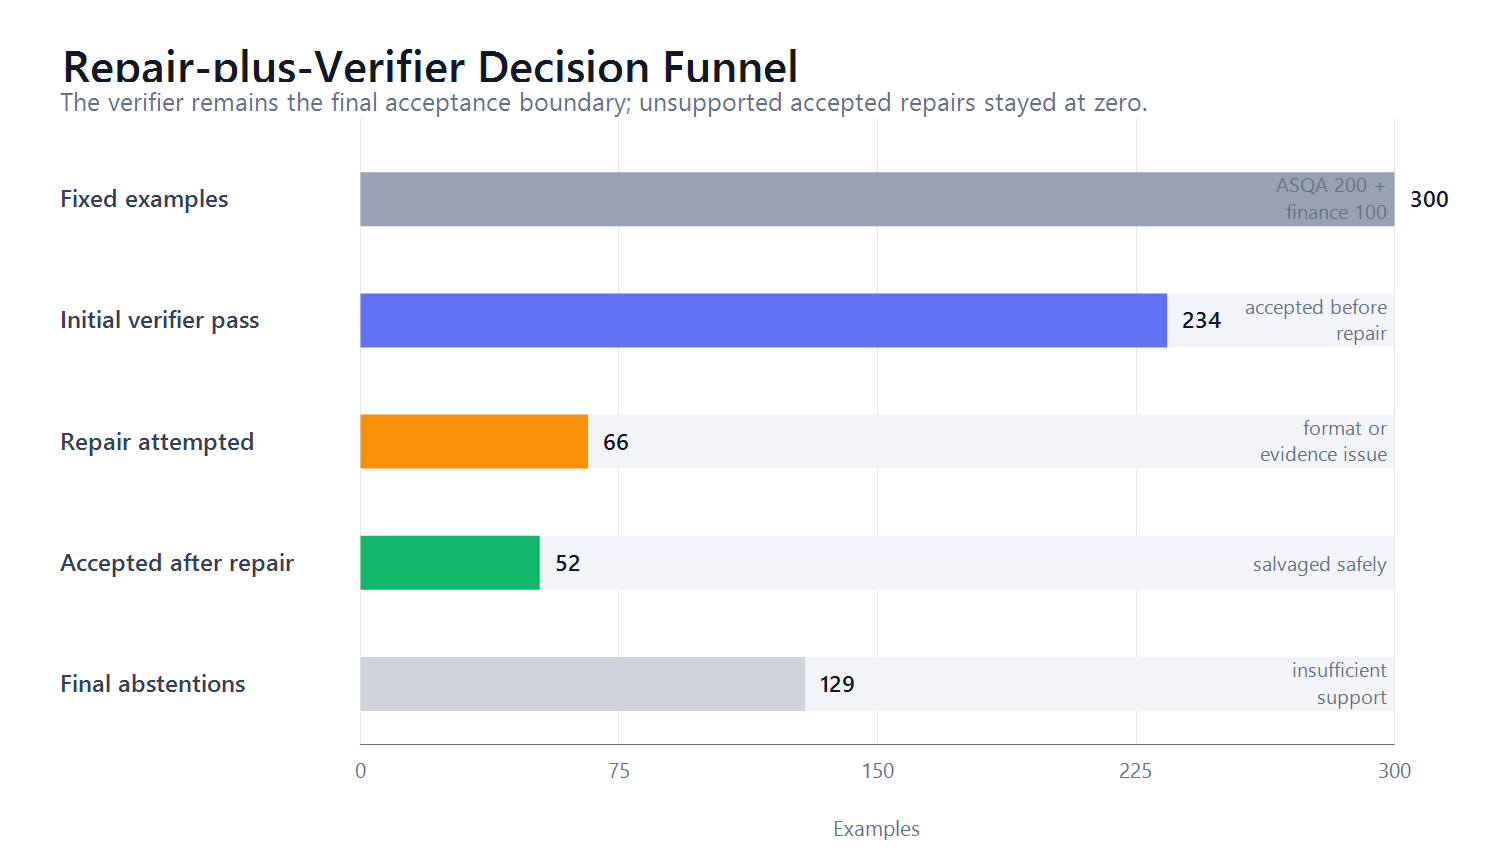
\includegraphics[width=0.98\textwidth]{assets/repair_funnel.png}
\caption{Repair-plus-verifier decision funnel from saved predictions. Repair is useful only when the verifier accepts the corrected answer; unsupported accepted repairs remained zero.}
\label{fig:funnel}
\end{figure*}

The generated distractor stress test adds a fourth irrelevant passage. Repair-plus-verifier 3B remains robust: ASQA obtains 55.0\% answer coverage with 0.0\% unsupported non-abstained answers, and finance obtains 85.0\% exact accuracy with 0.0\% unsupported non-abstained answers. This does not replace the fixed split; it is additional robustness evidence.

\section{Discussion and Limitations}
The strongest conclusion is narrow but useful. Verifier-bounded repair improves answer usefulness while preserving citation safety in this local setup. However, the ASQA verifier is a deterministic proxy rather than a human factuality audit. It checks citation structure and explicit anchors, but it does not prove complete semantic faithfulness. The finance dataset is synthetic, so it is a controlled stress test rather than real financial evidence. The 7B repair model was also much more conservative than 3B, especially on finance, where it abstained on all fixed examples.

Another limitation is that the attention gate was less important than the verifier and repair loop in the final result. The gate remains useful instrumentation, but the main contribution is the final verifier-bounded acceptance policy.

\section{Conclusion}
This project demonstrates a practical pattern for safer local RAG. A deterministic verifier can turn unsupported cited answers into explicit abstentions, and a one-step evidence-only repair loop can recover some supported answers without weakening that safety boundary. The best 3B repair-plus-verifier system achieves 0.0\% unsupported accepted answers on the fixed split, improves finance exact accuracy by 18 percentage points, and remains safe under a generated distractor stress test. The final repository includes source code, fixed splits, evaluation scripts, report tables, figures, qualitative examples, and reproducibility commands.

\begin{thebibliography}{9}
\bibitem{lewis2020rag}
P. Lewis et al., ``Retrieval-augmented generation for knowledge-intensive NLP tasks,'' NeurIPS, 2020.

\bibitem{asqa}
I. Stelmakh et al., ``ASQA: Factoid questions meet long-form answers,'' EMNLP, 2022.

\bibitem{alce}
T. Gao et al., ``Enabling large language models to generate text with citations,'' EMNLP, 2023.

\bibitem{jain2019}
S. Jain and B. C. Wallace, ``Attention is not explanation,'' NAACL, 2019.

\bibitem{wiegreffe2019}
S. Wiegreffe and Y. Pinter, ``Attention is not not explanation,'' EMNLP-IJCNLP, 2019.

\bibitem{ding2025}
Y. Ding et al., ``Attention attribution for generated text,'' ACL Findings, 2025.

\bibitem{qwen}
Qwen Team, ``Qwen2.5 technical report and model cards,'' 2024.

\end{thebibliography}

\end{document}
